\chapter{Conclusion}
\label{chap:conclusion}


\minitoc

Our concluding chapter summarizes our contributions, shows their complementarity
and discusses their possible evolutions.

Section~\ref{sec:conc:summary} summarizes our two contributions:
\toppi, an algorithm to mine efficiently association rules for any item in the dataset,
and \capa, a framework to study which quality measures
can highlight the most interesting association rules.

Section~\ref{sec:quali:pval} shows that item-centric results mined by \toppi
contain many associations of high interest according to Fisher's exact test.
This confirms the advantage of re-ranking each item's top itemsets according to a quality measure selected via \capa.

Section~\ref{sec:evolutions}
proposes three research directions that result from our work.


\section{Contributions summary}
\label{sec:conc:summary}

\subsection{Finding association rules about any item with \toppi}

The recent evolution of database systems allow the generation and storage
of transactional datasets containing hundreds of millions of transactions over millions of items.
Existing frequent itemsets mining algorithms cannot extract interesting results from such datasets,
even with the restriction to closed itemsets.
Indeed, by definition frequent itemsets only contain frequent items:
in our datasets of interest, this implies that results only cover the few frequent items.
The analyst may choose to increase the number of items considered frequent,
but this triggers a combinatorial explosion of results.

We therefore propose a new mining semantics,
where the analyst is only required to define the size of the desired output
using a single parameter, $k$.
Given $k$ we find,
for each item in the dataset,
the $k$ most frequent closed itemsets (CIS) containing this item.

Mining these top-$k$ CIS for all items at once provides the best amortization of each itemset's mining.
Our algorithm, \toppi, combines a dynamic enumeration of the frequent CIS space
with an efficient and fast pruning function.
We show that the combination of these two features is essential to find
per-item CIS in reasonable time.
We also show that mining item-centric CIS can be efficiently parallelized,
both on a multi-core server or on a Hadoop cluster,
in order to analyze large-scale datasets.

Not only \toppi is able to provide results which would be out of reach to existing methods,
but its item-centric approach also fits the way analysts usually browse association rules.
When the data concerns so many items,
she usually starts by picking an item she's familiar with, and search its associations.
She repeats this operation for other items,
as she progressively encounters new ones.
Thus \toppi provides the analyst with exhaustive and intuitively organized association rules.




\subsection{Choosing a quality measure to rank association rules with \capa}

When the distribution of items is highly unbalanced, as in our datasets of interest,
frequent associations may sometimes reflect artifacts.
Typically, a very frequent product like a shopping bag appears in almost all items' frequent associations.
But in most cases it does not really represent a link between the two products:
it only shows that everybody needs to carry groceries.
We can circumvent this phenomena by changing the sorting function of our associations.
But too many functions have been proposed in the literature,
from which we cannot judge which function is adequate to sorting associations in the retail domain.
Such artifacts occur in \toppi's results, but are also observed in more targeted studies,
for example when the analyst specifies a set of interesting items.
We therefore develop \capa, a framework to compare how \nbm quality measures rank association rules
extracted from 3 retail datasets.

We first perform an automatic comparison, by randomly picking 64 items,
mining their association rules and generating their \nbm ranked lists of associations.
Then we perform a hierarchical clustering, by comparing the rankings they produce.
Ranking similarity is measured using {\em Spearman's rank correlation},
Kendall's $\tau$, {\em Overlap@}$k$, and a novel one we propose: {\em NDCC}
(Normalized Discounted Correlation Coefficient).
This study allows us to distinguish 5 groups of measures.

In a second phase,
we ask marketing experts to evaluate a representative measure of each group.
We give them access to an association rules exploration application where they can choose
to rank rules according to one among 5 anonymized methods.
In all cases, analysts mentioned that ranking by decreasing {\em recall}
is uninteresting because it selects rules of too low {\em confidence}.
In general, sorting by decreasing {\em lift}
(which is close to sorting by decreasing {\em confidence})
is the preferred choice.
Combined with a minimum support threshold used in the mining phase,
this ranking promotes rules that are considered reliable.
However, the preference of the analysts changes when filters are available to narrow down the set of rules to specific product categories.
In this case, they favor the compromise between {\em confidence} and {\em support} offered, for instance,
by the {\em Piatetsky-Shapiro}'s measure~\cite{PiatetskyKDD91}.


\subsection{Industrial impact}

This work has been conducted in the context of \datalyse, an industrial project.
Our industrial partners provide the infrastructure for the joined analysis of three data sources:
supermarket receipts, customer information and a taxonomy of products.
End-users are marketing analysts who need to
study the associations between products,
or between customers and products.

Thanks to our collaboration with Intermarch\'e we could work on real data,
following realistic use cases of analytics in the retail domain.
We also benefited from the feedback of marketing experts
when evaluating the results produced both by \toppi and \capa.

Our contributions were also progressively integrated in the production workflow of Intermarch\'e.
This started with our earliest work, \jlcm,
our implementation of PLCM~\cite{NegrevergneHPCS10} in Java.
\toppi was also delivered,
which led Intermarch\'e to propose the improvements detailed in
Section~\ref{sec:toppi:integration} (p.\pageref{sec:toppi:integration}).
This motivated the development of \capa,
which involved experts from the marketing studies department of Intermarch\'e.
The final version of \toppi, deployed in production,
includes a post-processing:
instead of being ranked by decreasing frequency,
each item's itemsets are ranked by decreasing correlation with the item,
according to the $p$-value.
The following experiment shows that this post-processing allows our miner
to return smaller lists of more relevant itemsets per item.


\section{Improving \toppi by re-ranking per-item closed itemsets}
\label{sec:quali:pval}


\toppi relies only on support to select the top-$k$ CIS containing an item.
In this section we show that it is sufficient to find the top results per-item
according to a finer quality measure:
the $p$-value, computed with Fisher's exact test as described in Annex~\ref{chap:fisher} (p.\pageref{chap:fisher}).

%thus providing results that can fit in \capa.
Ranking by decreasing frequency allows \toppi  to efficiently traverse a small portion of the CIS space,
as shown in Chapter~\ref{chap:toppi}.
%An item's itemsets can be converted to association rules by removing the item from each one.
Although it provides valuable results,
\toppi's output also contains a few uninteresting associations:
the most frequent items appear too often with long-tail items.
Our experiments with \capa suggest that some scoring functions
(from $G_3$, see Table~\ref{tab:measures} p.\pageref{tab:measures})
may allow the automatic extraction of more interesting itemsets for each item.
% To the best of our knowledge,
% there is no algorithm able to directly extract from our datasets
% the top-$n$ CIS of each item according to one of these measures.
% Indeed, guaranteeing that the output's scores dominate all others in the solutions space
% requires the exploration of too many itemsets.
The traditional approach
(and the most efficient in our case, see Section~\ref{sec:rel:lamp}, p.\pageref{sec:rel:lamp})
to mine association rules with both high {\em support} and {\em confidence} is to first extract frequent CIS,
then filter them using a {\em confidence} threshold~\cite{AgrawalVLDB94}.
In a similar fashion,
we propose to re-rank \toppi's results (for each item) to obtain high quality item-centric association rules.

From here we note top-$k$ when itemsets are sorted by decreasing frequency (as in \toppi),
and top-$n$ when itemsets are sorted according to a finer quality measure (as in \capa).
To assess the relevance of our re-ranking strategy,
we measure in the following experiment how \toppi's results contain
the top-$n$ itemsets per-item according to the representative measure of $G_3$: Fisher's exact test.
The bound described by Minato {\em et al.}~\cite{MinatoKDD14}
allows us to find a minimum frequency threshold ensuring that
the candidate CIS mined to generate each top-$n$ do have a better $p$-value than any other.

\begin{figure}
	\centering
  \begin{tabular}{cc}
		\begin{subfigure}[b]{0.48\textwidth}
			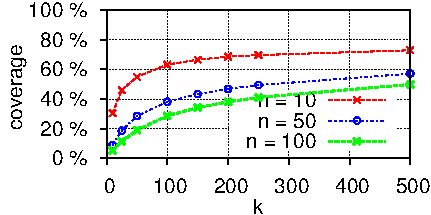
\includegraphics{fig/toppi/top-Correlatedcoverage/tickets2013.pdf}
			\caption{\prodassocreceipt}
		\end{subfigure}
  	&
  	\begin{subfigure}[b]{0.48\textwidth}
  		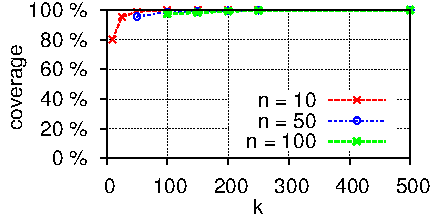
\includegraphics{fig/toppi/top-Correlatedcoverage/supermarket.pdf}
  		\caption{\em Supermarket}
  	\end{subfigure}
    \\
		\begin{subfigure}[b]{0.48\textwidth}
  		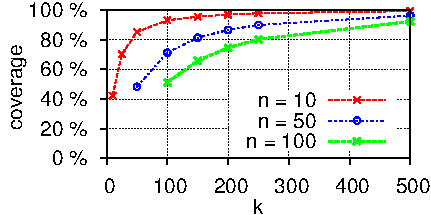
\includegraphics{fig/toppi/top-Correlatedcoverage/lastfm.pdf}
  		\caption{\em LastFM}
  	\end{subfigure}
    &
    \begin{minipage}[b]{0.40\linewidth}
    \vspace{-2in}
      \caption{\label{fig:pvalCoverage}
    		\toppi's output coverage of the top-$n$ by $p$-value
    	}
    \end{minipage}
    \\
  \end{tabular}
\end{figure}

This may still require the generation of millions of itemsets per item.
Hence we perform this experiment on a sample of the items from our datasets.
We generate 10 buckets of items according to their support,
and randomly select 50 items in each, for a total of 500 items.
For each selected item $i$,
we mine frequent CIS in ${\cal D}_{i} = \langle t \setminus \{i\} \mid t \in {\cal D}, i \in t\rangle$.
Then we measure the correlation of occurrences of these CIS with occurrences of $i$ in $\cal D$.
Finally we rank the CIS by increasing $p$-value, thus obtaining the item's top-$n$.
Figure~\ref{fig:pvalCoverage} shows \toppi's output coverage of the ground truth we generated,
for various $k$ and $n$.

For supermarket tickets,
this experiment shows that the majority of the sampled items' top-$n$ CIS are contained in \toppi's top-$k$ lists.
However, results are extremely different if the experiment is done on the complete dataset,
\prodassocreceipt, or on its preliminary version, {\em Supermarket}.
This is all the more surprising as these two datasets have very similar items distributions.
But, at this scale (\prodassocreceipt is 10 times larger than {\em Supermarket}),
some extremely rare associations may have an artifically strong $p$-value
and are not mined by \toppi.

For \textit{LastFM},
at coordinates $k=100$ we can see that the top-$k$ of an item contains on average $93\%$
of the itemsets of its top-$n$ (by $p$-value) for $n=10$, $71\%$ for $n=50$, and $51\%$ for $n=100$.
With this dataset, \toppi's coverage of the top-by-$p$-value is above $90\%$ for $k \ge 5n$.
This means that, when $k \ge 5n$,
for the sampled items $90\%$ of the top-$n$ (by $p$-value) CIS appear in \toppi's top-$k$ (by frequency).
Therefore, if we re-rank \toppi's results by $p$-value,
the final lists would be quite close to the exact top-$n$.
This is interesting, because computing the exact top-$n$ is much more costly.

For this reason, we cannot show results for \prodassocclient.
In this dataset, computing the sampled items' top-$n$ by $p$-value is too complex
and would require several months of CPU time.
Because its transactions are around 10 times longer than in \prodassocreceipt,
the number of frequent CIS explodes quickly.
Therefore, guaranteeing the result's correctness sometimes requires the mining and storage of billions of itemsets.
Similarly, computing the ground truth for only 500 items of {\em LastFM} takes 8.6 hours of CPU time.
On the same dataset, \toppi consumes 3.1 hours of CPU for all the \num{450000} items and the highest value of $k$.

Overall, this confirms that \toppi can be used as part of a two-step approach to accurately emulate refined,
but computationally costly, interestingness measures on large-scale datasets.
It is currently in use at Intermarch\'e.
%Our user study (p.\pageref{sec:xp:user}) and the previous difficulties with Fisher's exact test suggest
%that the per-item CIS found by \toppi can be re-ranked using  {\em Piatetsky-Shapiro}'s measure~\cite{PiatetskyKDD91}.
Thanks to this approach,
extracting association rules from a large collection of transactions is both affordable and interesting for a nation-wide retailer,
that would otherwise have to ask experts to filter manually the input or the results~\cite{SuganthanSIGMOD15}.







\section{Towards an interactive associations explorer}
\label{sec:evolutions}

We conclude by describing potential evolutions of our contributions.
These would improve the system's response time,
the quality of its results and
its reactivity to the continuous updates usually performed on modern datasets.

\subsection{Shortening computation batches}

Both \jlcm, \capa and \toppi are implemented using batch processing and on-disk storage.
While mining is already fast,
I/O operations introduce some latency (sometimes measured in hours)
between the definition of a mining scenario and the display of results.
Thanks to the evolution of memory technologies,
at the time of writing our datasets can fit in a single server.
The curation step of our workflow could be executed efficiently in minutes or less
using an in-memory database~\cite{lindstrom2013ibm,LeeICDE13}.

For an even faster processing, or larger datasets,
we could also rely on an in-memory distributed dataset representation.
For example, Spark proposes the {\em Resilient Distributed Datasets}~\cite{ZahariaHC10},
which have been massively adopted by industry and academia,
and improved since~\cite{ArmbrustSIGMOD15}.
Spark would also speed up the distributed variant of \toppi,
but not significantly because the local mining done by each worker remains the major time bottleneck.

The ability of large-scale in-memory systems to obtain small selections or samples of a dataset
almost instantly also makes them necessary to a more interactive mining process,
as proposed in the following sections.



%The first step would be the transition of a prepared transactions step in the cluster's cache.
%As users are usually applying narrow filters over the products' taxonomy,
%each filter could be transposed as a constraint for \algo.
%With such constraints,  association rules can be computed in less than a second.
%
%A second step would be moving the whole receipts database to an in-memory cluster,
%though that would be much more storage-consuming.



\subsection{Adaptive mining and ranking}
\label{sec:evolutions:adaptative}

In~\cite{LiuICDE11}, Liu \textit{et al.} propose an association rules exploration framework
where rules are grouped by consequent,
then traversed by progressively adding items to the antecedent.
The framework provides hints on how each additional item would make a difference.
Such a framework is suitable to the scenarios we consider,
and would improve our association rules exploration.
It would also drastically restrict the CIS enumeration,
because at each step the system would only have to traverse direct extensions of current associations.
%It would also us to dynamically generate filtering rules,
%to eliminate products that are deemed irrelevant by the analysts.

This iterative approach would also allow the system to learn the user's preference for ranking associations~\cite{dzyubaIJAIT14}.
Each interaction would allow the system to refine its understanding of the analyst's needs,
and in particular its notion of interesting association.


\subsection{Mining as we explore}

A dynamic definition of interesting associations would shorten mining time,
because we would only have to traverse the small portion of the CIS space pointed out by the analyst.
But with large datasets this may not be enough to reach sub-second response times,
in particular when most transactions contain more than a thousand items.
In our work,
the greatest mining times are observed with {\em WebDocs},
which has the longest transactions (177 items, on average).
Should they contain ten or a hundred times more items,
the datasets would be out of reach of \toppi.
In these cases, mining closed itemsets is too precise to be efficient:
we have to count precisely the occurrences of each item or itemset in each transaction,
which is too costly when transactions are too long.

To avoid this, the iterative process described in Section~\ref{sec:evolutions:adaptative} may include an intermediate step.
The system would firstly approximate the itemsets or their support,
and mine precisely only once the analyst has shown interest for the result.
For instance, PARMA~\cite{RiondatoCIKM12} shows that we can get a reliable approximation of frequent itemsets,
in distributed datasets, using distributed sampling.



\begin{paragraph}{}
	Thanks to the improvements proposed in this section,
	the system would be able to provide insightful results for large scale datasets
	using much less CPU time.
	As large-scale datasets are evolving continuously,
	it will be more and more relevant to only explore the portion of the CIS space which is interesting to the analyst at the time she's using it.
	%hence we may not have to generate a complete snapshot of associations every time
	%millions of transactions do not appear on a single day.
\end{paragraph}
